% Golden Spiral can be approximated with Golden ratio or Fibonacci sequence.
% Golden Ratio: a+b/a = a/b

\documentclass{beamer}
\usepackage[utf8]{inputenc}
\usepackage[T1]{fontenc}

\usepackage{hyperref}
\usepackage{graphicx}
\hypersetup{
    colorlinks=true,
    linkcolor=blue,
    filecolor=magenta,      
    urlcolor=cyan,
}

\usetheme{Cuerna}
\usecolortheme{default}
% default, bluesimplex, lettuce, brick

% slide (frames) numbering
% \addtobeamertemplate{navigation symbols}{}{
%     \usebeamerfont{footline}%
%     \usebeamercolor[fg]{footline}%
%     \hspace{1em}%
%     \insertframenumber/\inserttotalframenumber
% }

\title{Action Robust Reinforcement Learning and Applications in Continuous Control}
\author{Shayan Amani}

\date{September 26, 2019}
\institute{Department of Computer Science, University of New Hampshire}

\begin{document}

  \begin{frame}
    \titlepage
  \end{frame}

\begin{frame}
    \frametitle{Action Robustness}
        Robustness in action selection:
            \begin{enumerate}
                \item Perturbation in policy space.
        
        \begin{equation} \tag{1}
            \pi_{P, \alpha}^{\operatorname{mix}}(\mathbf{a} |\mathbf{s}) \equiv(1-\alpha) \pi(\mathbf{a} | \mathbf{s})+\alpha \overline{\pi}(\mathbf{a} | \mathbf{s})
        \end{equation}
             \end{enumerate}
\end{frame}

\begin{frame}
    \frametitle{Action Robustness}
        Robustness in action selection:
            \begin{enumerate}
                \item Probabilistic perturbation in policy space.
        
                    \begin{equation} \tag{1}
                        \pi_{P, \alpha}^{\operatorname{mix}}(\mathbf{a} |\mathbf{s}) \equiv(1-\alpha) \pi(\mathbf{a} | \mathbf{s})+\alpha \overline{\pi}(\mathbf{a} | \mathbf{s})
                    \end{equation}
        
                \item {[Probabilistic]} perturbation in action space.
                    \begin{equation} \tag{2}
                        \pi_{N, \alpha}^{\operatorname{mix}}(\mathbf{a} | \mathbf{s}) \equiv \mathbb{E}_{\mathbf{b} \sim \pi(\cdot | s)}\left[\mathbf{1}_{\mathbf{a}=(1-\alpha) \mathbf{b}+\alpha \overline{\mathbf{b}}}\right]
                    \end{equation}
        
             \end{enumerate}
\end{frame}



\begin{frame}
    \frametitle{Approaches}

    PR-MDP \\\\
    \begin{equation}
        \pi_{P, \alpha}^{*} \in \underset{\pi \in \mathcal{P}(\Pi)}{\arg \max } \min _{\overline{\pi} \in \Pi} \mathbb{E}^{\pi_{P, \alpha}^{\operatorname{mix}}(\pi, \overline{\pi})}\left[\sum_{t} \gamma^{t} r\left(\mathbf{s}_{t}, \mathbf{a}_{t}\right)\right]
    \end{equation}
    
    NR-MDP \\\\
    \begin{equation}
        \pi_{N, \alpha}^{*} \in \underset{\pi \in \mathcal{P}(\Pi)}{\arg \max } \min _{\overline{\pi} \in \Pi} \mathbb{E}^{\pi_{N, \alpha}^{\operatorname{mix}}(\pi, \overline{\pi})}\left[\sum_{t} \gamma^{t} r\left(\mathbf{s}_{t}, \mathbf{a}_{t}\right)\right]
    \end{equation}
  \end{frame}



\begin{frame}
    \frametitle{PI Variants}
        \begin{figure}
            \centering
            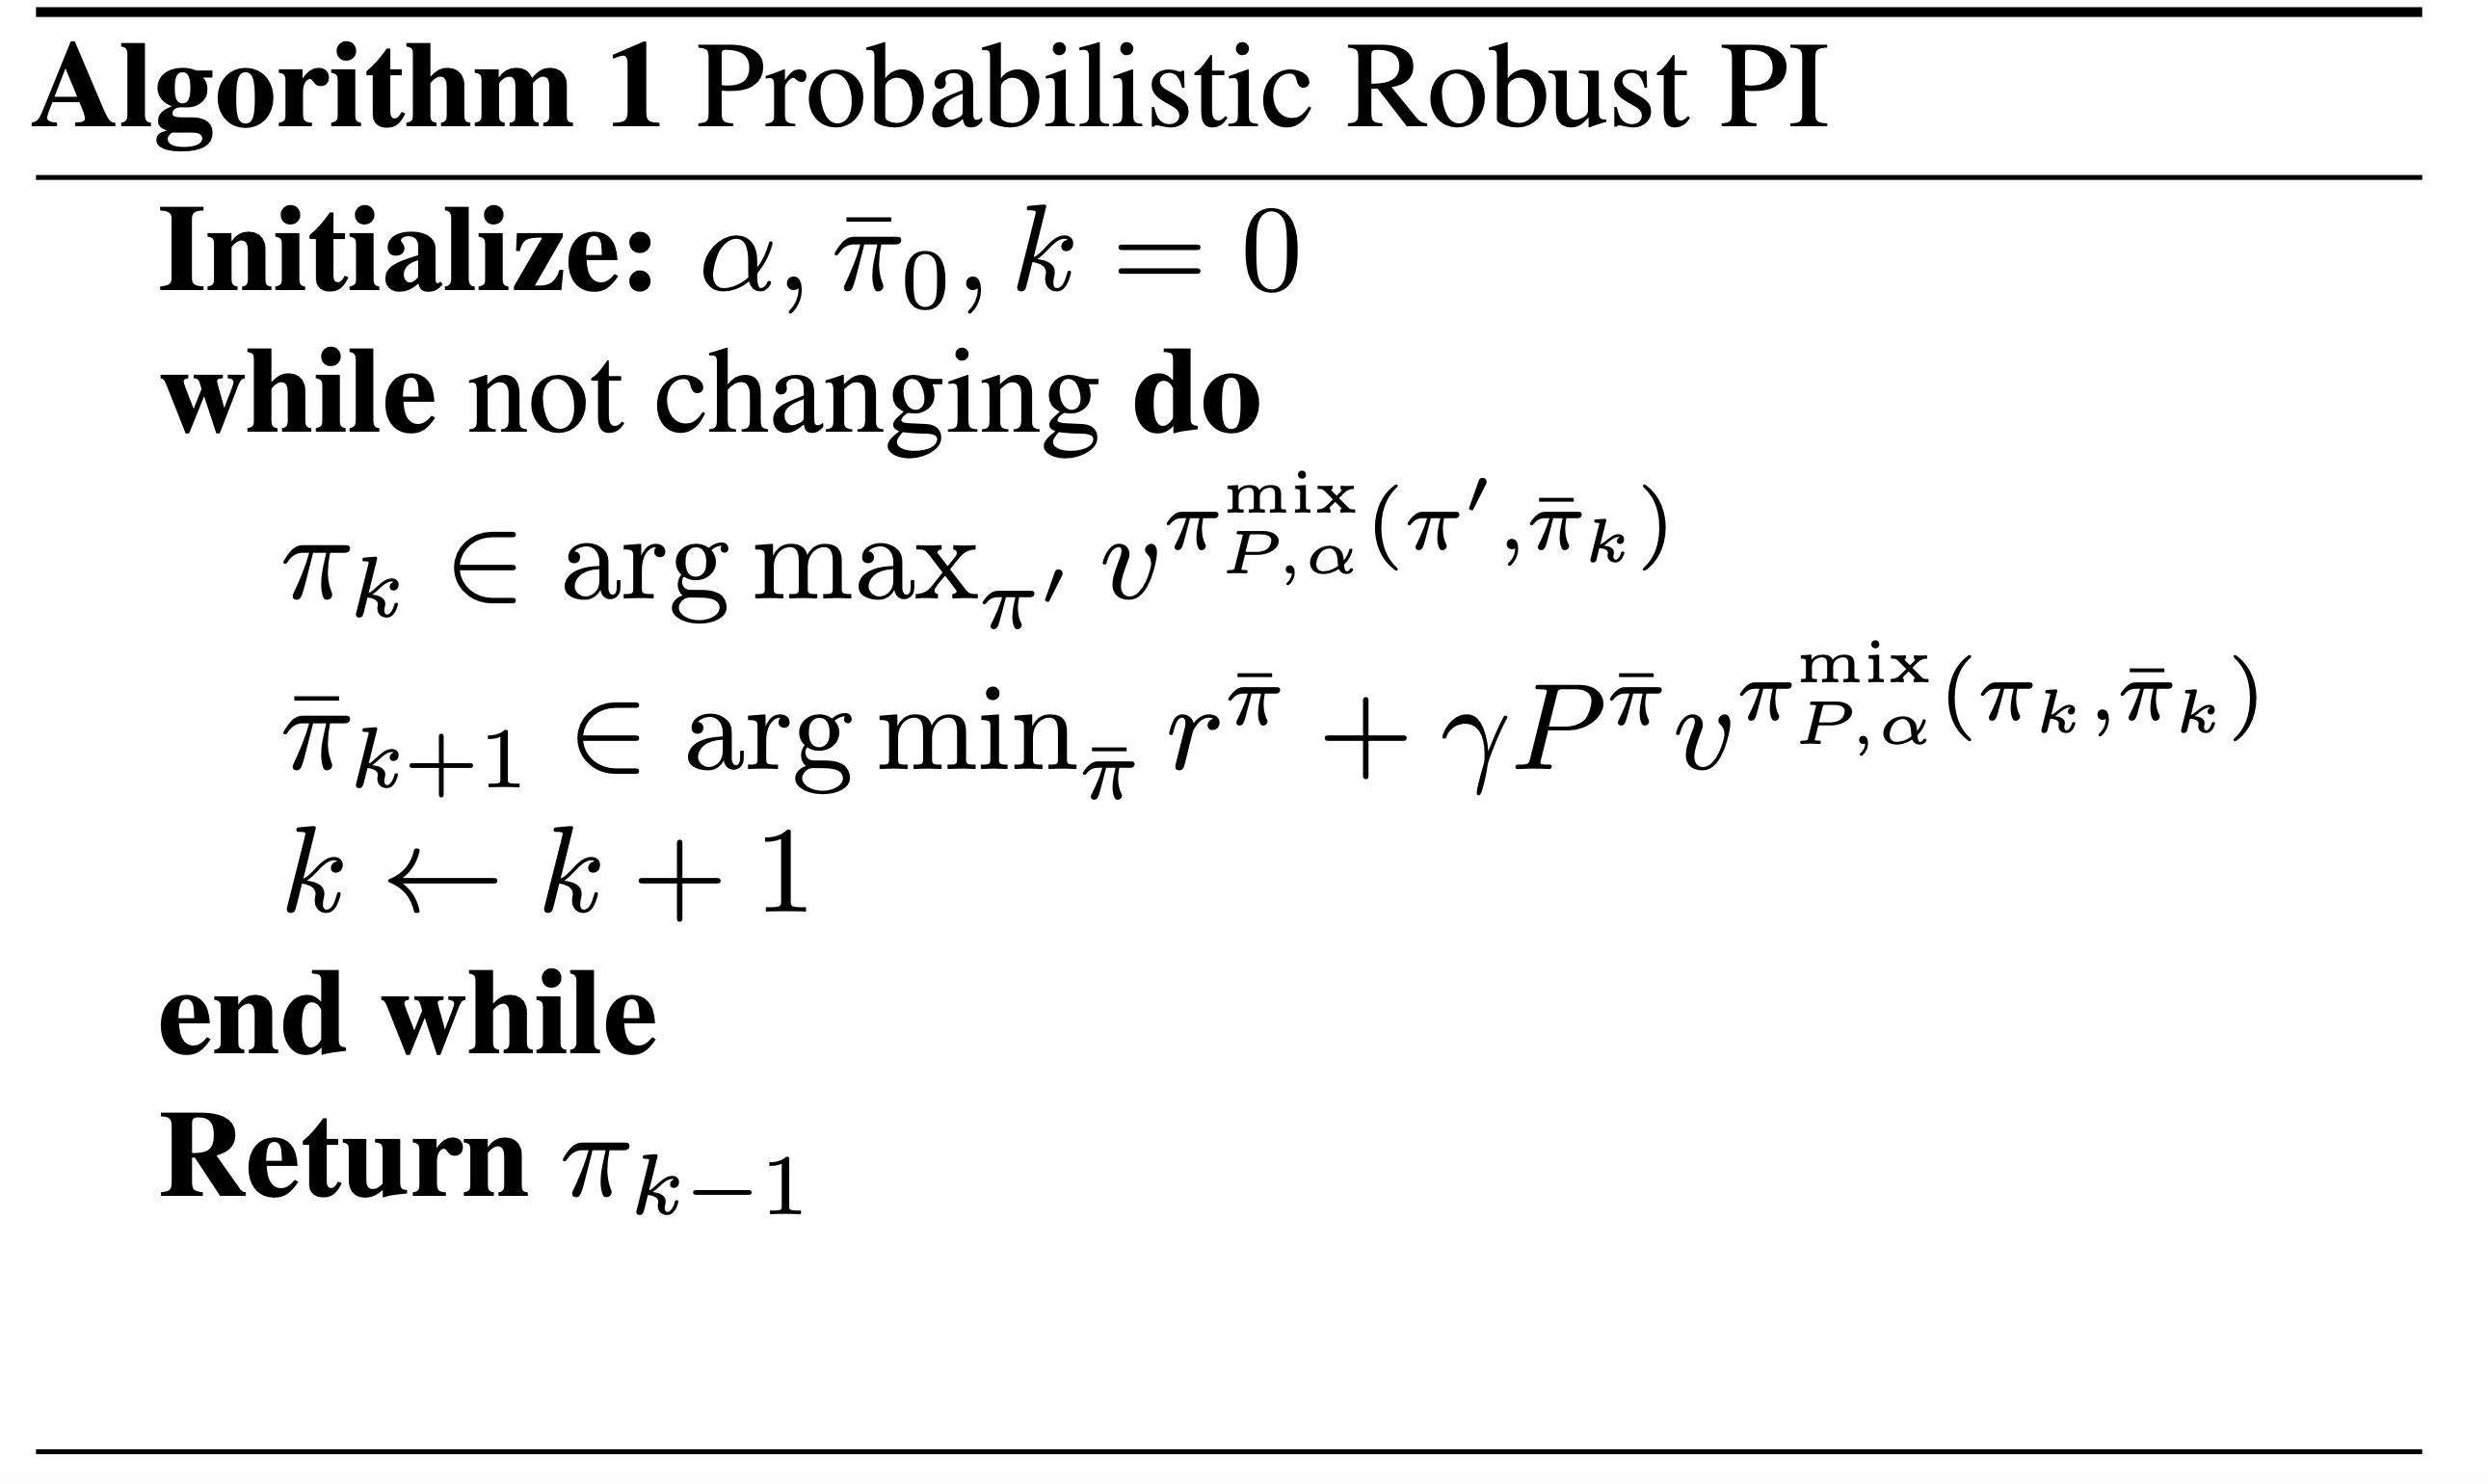
\includegraphics[scale=0.115]{alg1.png}
    	    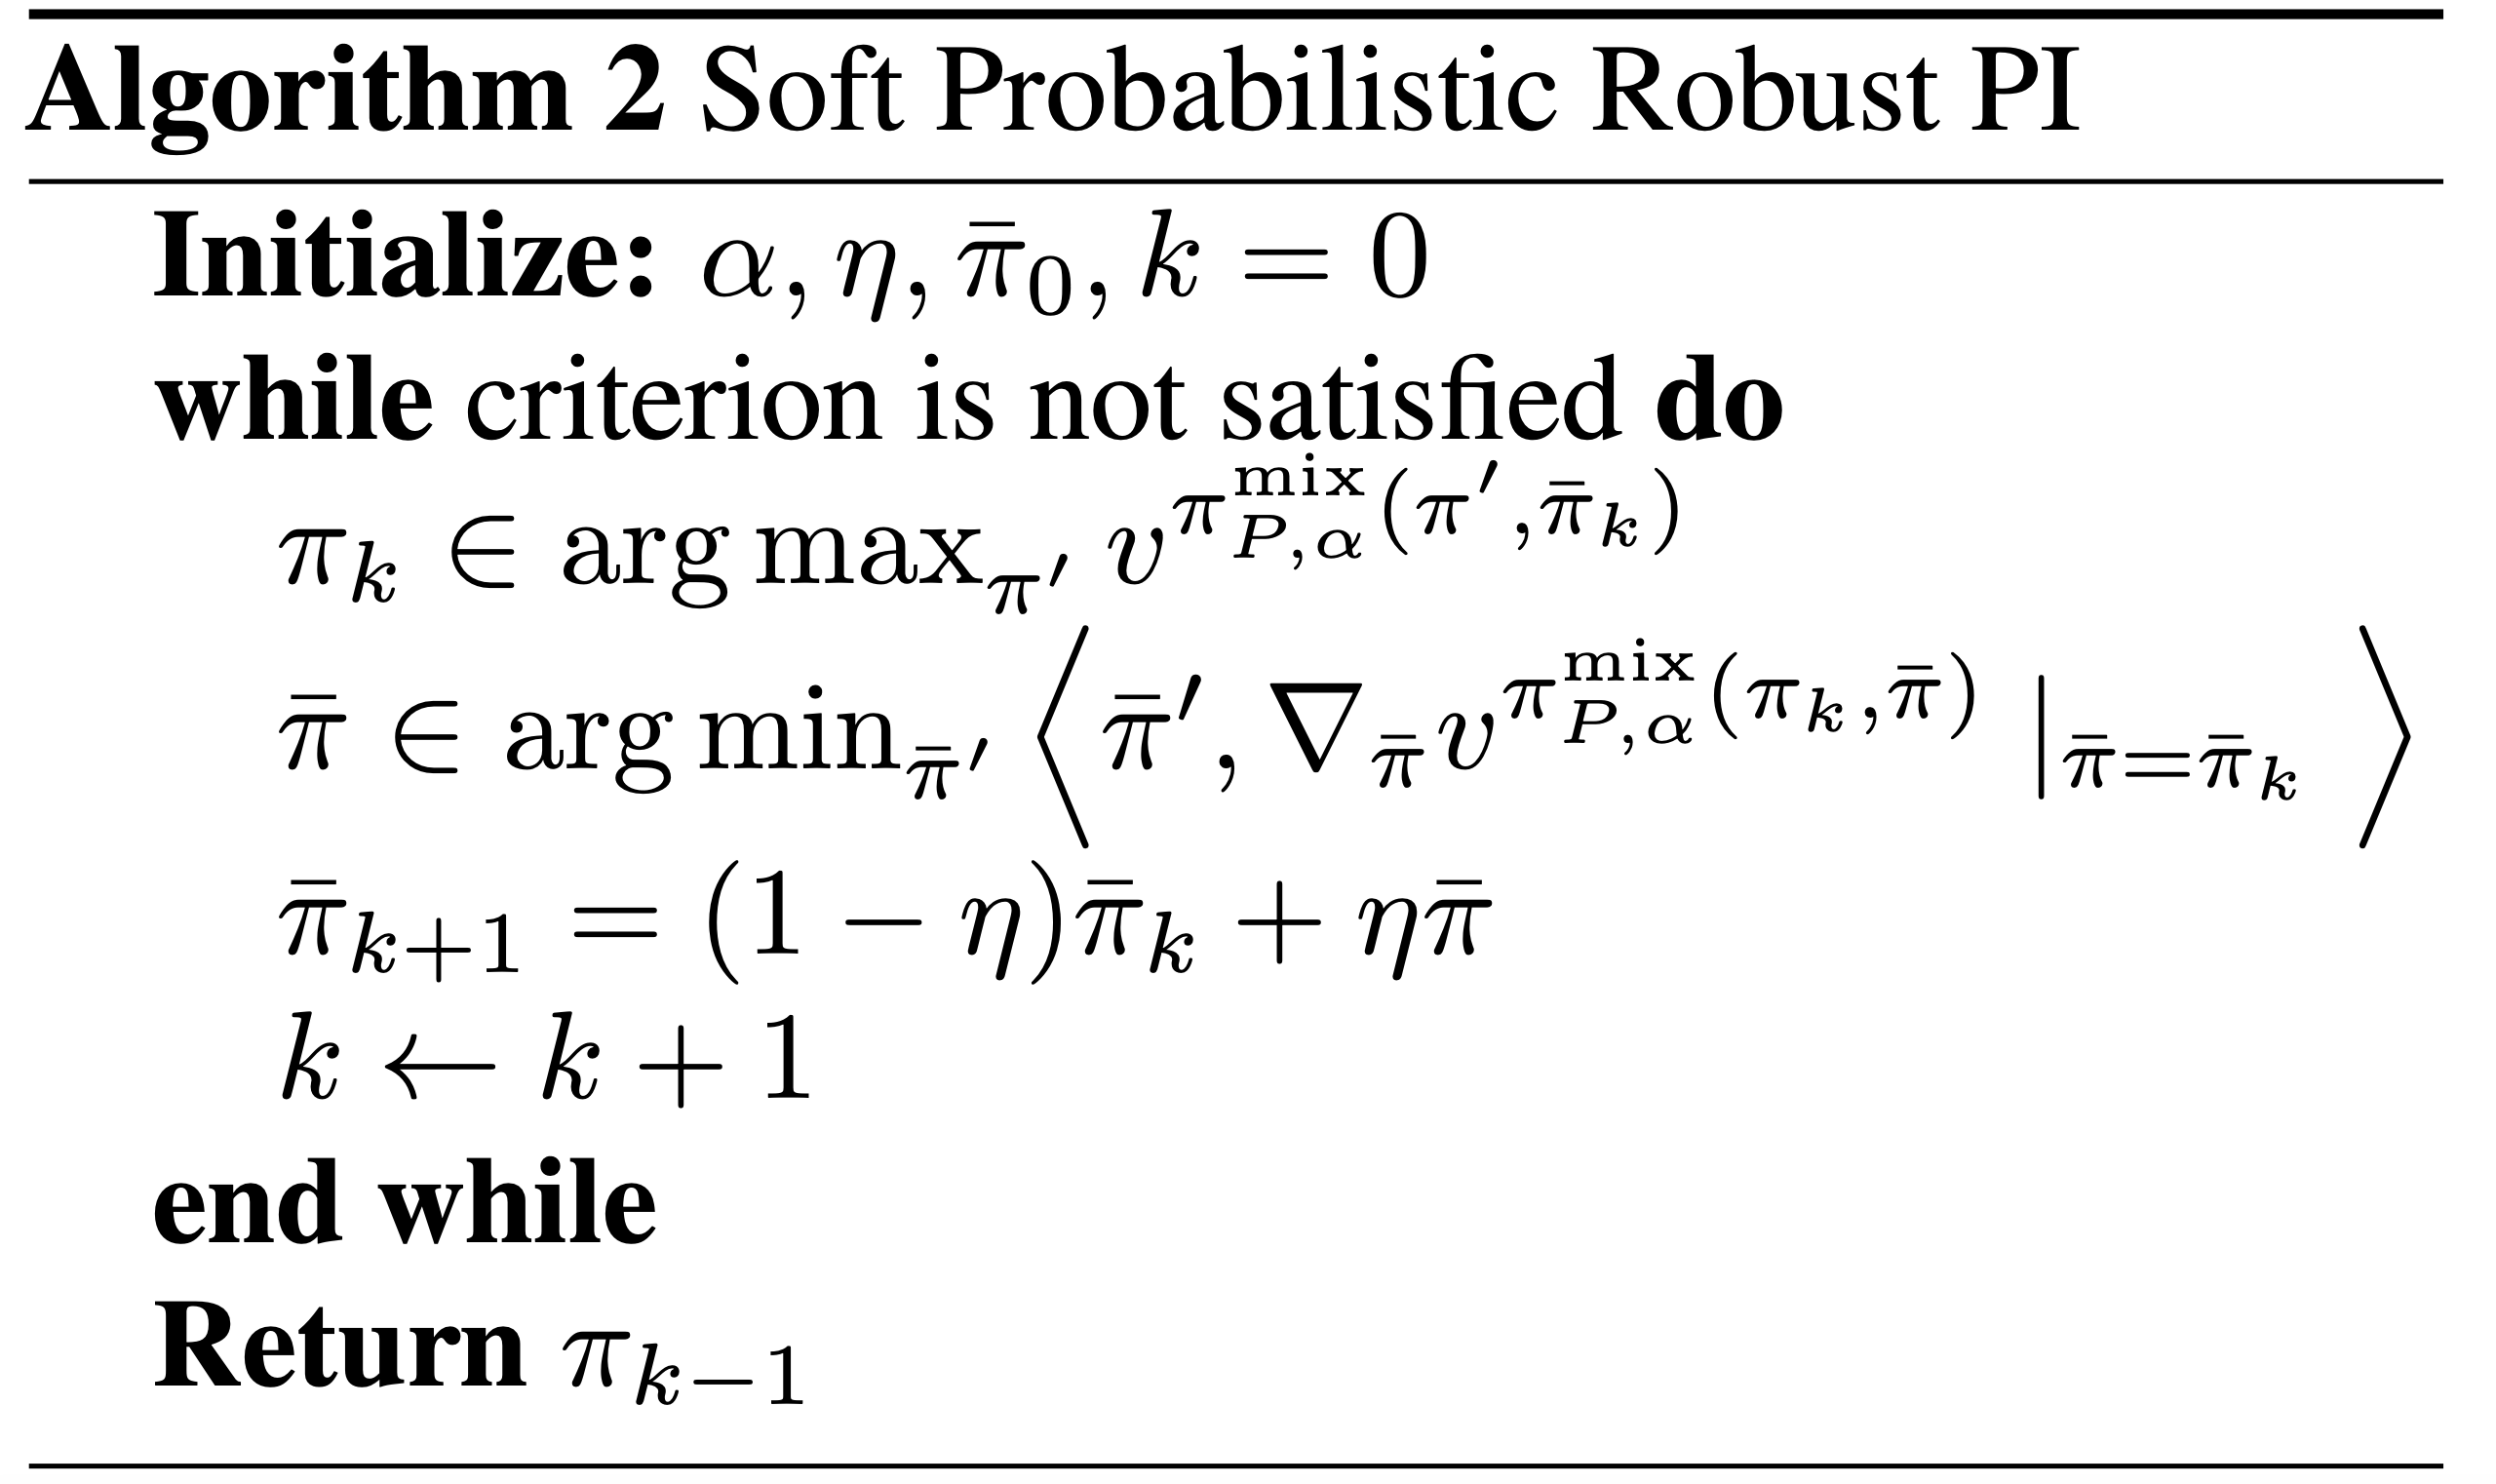
\includegraphics[scale=0.115]{alg2.png}
            \label{fig:my_label}
        \end{figure}
    	
\end{frame}


\begin{frame}
       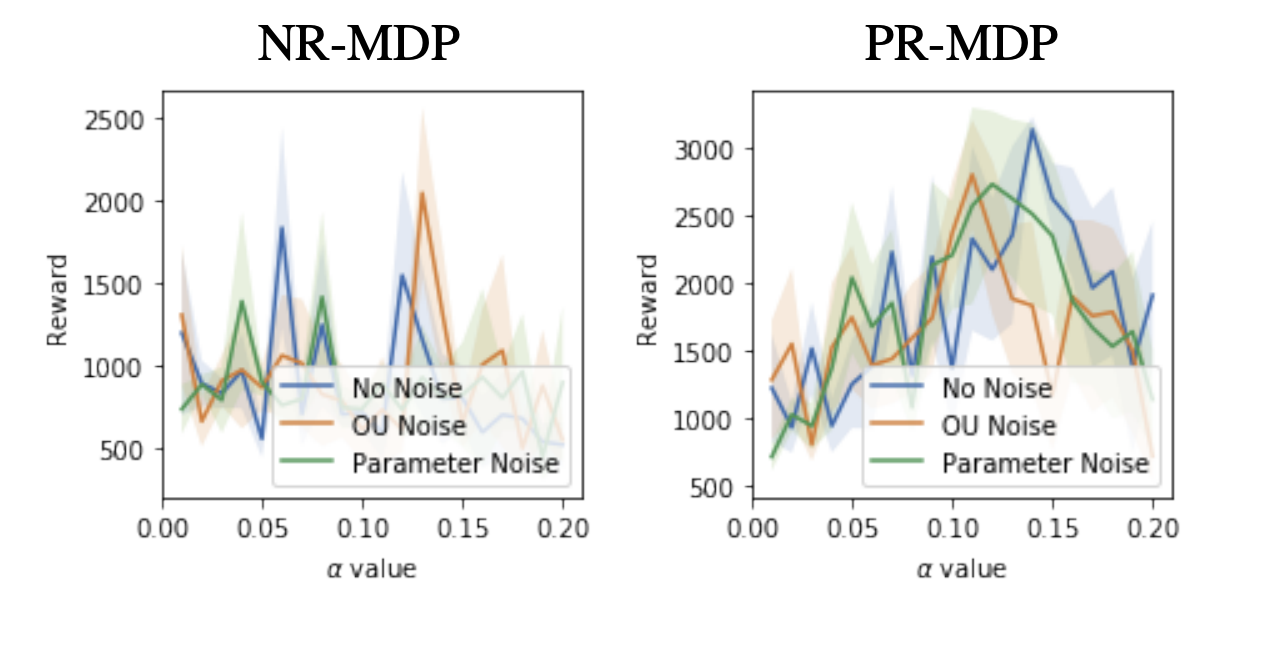
\includegraphics[width=1\columnwidth]{noisy.png}
\end{frame}


\begin{frame}
       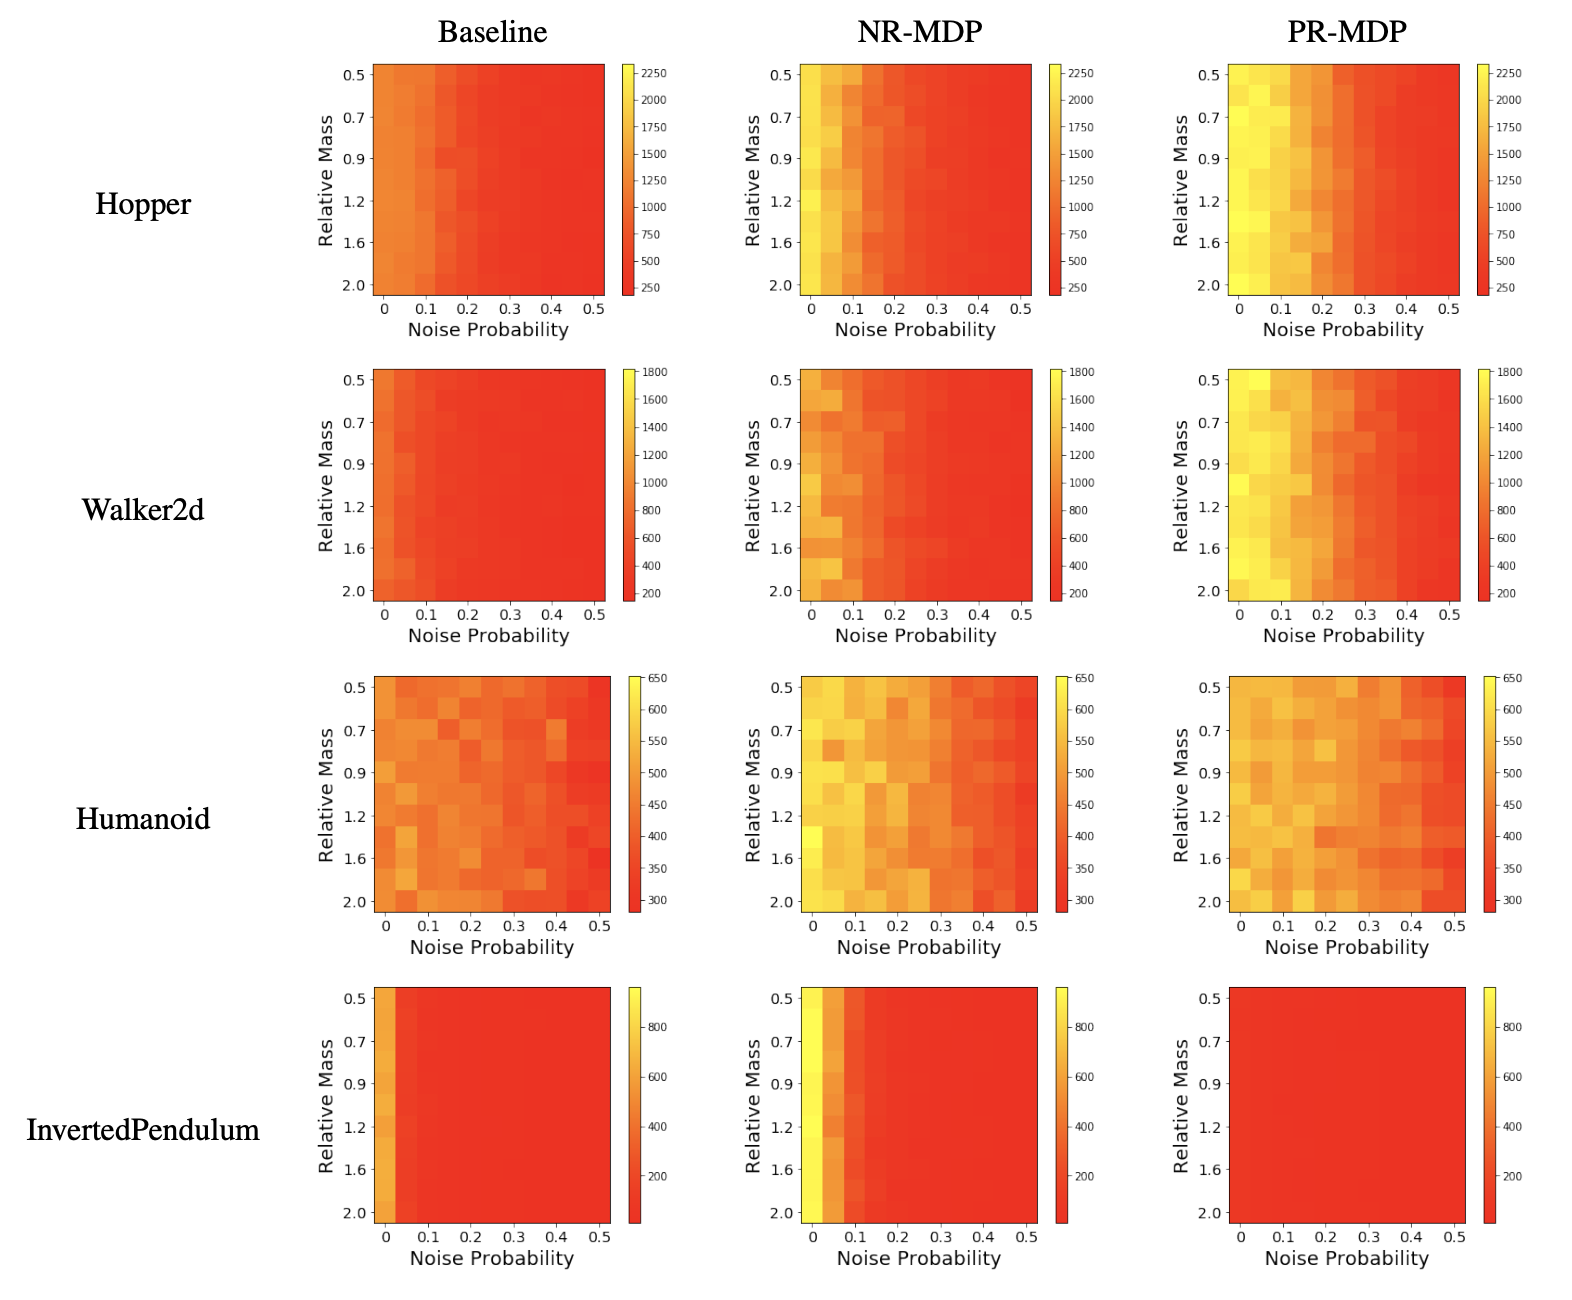
\includegraphics[width=1\columnwidth]{heatmap.png}
\end{frame}

\end{document}